\documentclass{article}

% content/resources/templates/preamble.tex
\usepackage[margin=0.6in]{geometry}
\author{Milav Dabgar}
\usepackage{amsmath,amssymb,amsthm}
\usepackage{booktabs}
\usepackage{multirow}
\usepackage{xcolor}
\usepackage{tcolorbox}
\tcbuselibrary{breakable,skins}
\usepackage[colorlinks=true,linkcolor=blue]{hyperref}
\usepackage{titlesec}
\usepackage{enumitem}
\usepackage{tikz}
\usepackage{pgfplots}
\usepackage{circuitikz}
\usepackage[version=4]{mhchem}
\usepackage{longtable}
\usepackage{array}
\usepackage{float}
\usepackage{caption}
\usepackage{listings}

\lstset{
  basicstyle=\small\ttfamily,
  breaklines=true,
  breakatwhitespace=false,
  postbreak=\mbox{\textcolor{red}{$\hookrightarrow$}\space},
  float=false,
  numbers=left,
  numberstyle=\tiny\color{gray},
  numbersep=10pt,
  xleftmargin=2em,
  keywordstyle=\color{blue},
  commentstyle=\color{green!60!black},
  stringstyle=\color{purple},
  backgroundcolor=\color{gray!5},
  showstringspaces=false,
  tabsize=2,
  captionpos=b,
  keepspaces=true,
  columns=flexible
}

\pgfplotsset{compat=1.18}
\usetikzlibrary{shapes,arrows,positioning,calc,patterns,decorations.pathmorphing,decorations.markings,arrows.meta}

% Color scheme
\definecolor{headcolor}{RGB}{0,102,204}
\definecolor{keycolor}{RGB}{220,20,60}
\definecolor{solutioncolor}{RGB}{34,139,34}
\definecolor{mnemoniccolor}{RGB}{148,0,211}
\definecolor{codecolor}{RGB}{0,0,100}

% Spacing
\setlength{\parskip}{3pt}
\setlist[itemize]{nosep}
\setlist[enumerate]{nosep}

% Title formatting
\titleformat{\section}{\Large\bfseries\color{headcolor}}{\thesection}{1em}{}
\titleformat{\subsection}{\large\bfseries\color{headcolor}}{\thesubsection}{1em}{}

% Pandoc tightlist compatibility
\providecommand{\tightlist}{%
  \setlength{\itemsep}{0pt}\setlength{\parskip}{0pt}}

% Pandoc longtable compatibility
\newcounter{none}
\def\thenone{}


% content/resources/templates/english-boxes.tex

% Custom environments
\newtcolorbox{solutionbox}{
 breakable,
 enhanced,
 colback=solutioncolor!5!white,
 colframe=solutioncolor!75!black,
 fonttitle=\bfseries,
 title=Solution
}

\newtcolorbox{solutionboxnobreak}{
 colback=solutioncolor!5!white,
 colframe=solutioncolor!75!black,
 fonttitle=\bfseries,
 title=Solution
}

\newtcolorbox{keyformula}{
 breakable,
 enhanced,
 colback=keycolor!5!white,
 colframe=keycolor!75!black,
 fonttitle=\bfseries,
 title=Key Formula
}

\newtcolorbox{mnemonicboxenv}{
 breakable,
 enhanced,
 colback=mnemoniccolor!5!white,
 colframe=mnemoniccolor!75!black,
 fonttitle=\bfseries,
 title=Mnemonic
}

\newcommand{\mnemonicbox}[1]{%
  \begin{mnemonicboxenv}
    #1
  \end{mnemonicboxenv}
}


% Custom commands for GTU solutions
% This file defines semantic commands for consistent formatting

% Question command with automatic formatting
\newcommand{\question}[2]{%
  \section*{Question #1}%
  \textbf{#2}%
}

% OR question variant
\newcommand{\questionor}[2]{%
  \section*{Question #1 OR}%
  \textbf{#2}%
}

% Proper table environment with caption
\newenvironment{answertable}[1]{%
  \begin{table}[htbp]
  \centering
  \caption{#1}
}{%
  \end{table}
}

% Proper figure environment for diagrams
\newenvironment{answerdiagram}[1]{%
  \begin{figure}[htbp]
  \centering
  \caption{#1}
}{%
  \end{figure}
}

% Semantic markup for key terms
\newcommand{\keyword}[1]{\textbf{#1}}
\newcommand{\code}[1]{\texttt{#1}}
\newcommand{\classname}[1]{\texttt{#1}}
\newcommand{\methodname}[1]{\texttt{#1}}

% Proper quotation marks
\newcommand{\mnemonic}[1]{``#1''}


\title{Embedded System \& Microcontroller Application (4351102) - Summer 2025 Solution}
\date{May 12, 2025}

\begin{document}
\maketitle

\questionmarks{1(a)}{3}{State the features of ATmega32.}

\begin{solutionbox}
\textbf{ATmega32 Features:}

\begin{answertable}{ATmega32 Features}
\begin{tabulary}{\linewidth}{|L|L|}
\hline
\textbf{Feature} & \textbf{Description} \\ \hline
\keyword{Flash Memory} & 32KB programmable memory \\ \hline
\keyword{SRAM} & 2KB internal SRAM \\ \hline
\keyword{EEPROM} & 1KB non-volatile data storage \\ \hline
\keyword{I/O Pins} & 32 programmable I/O lines \\ \hline
\keyword{Timers} & 3 flexible timer/counters \\ \hline
\keyword{ADC} & 10-bit 8-channel ADC \\ \hline
\end{tabulary}
\end{answertable}

\keyword{Additional Specifications:}
\begin{itemize}
    \item \keyword{Operating Voltage}: 2.7V to 5.5V range
    \item \keyword{Clock Speed}: Up to 16 MHz operation
    \item \keyword{Communication}: USART, SPI, I2C interfaces
\end{itemize}
\end{solutionbox}

\begin{mnemonicbox}
\mnemonic{Fast SRAM Enjoys Input Timers And Communication}
\end{mnemonicbox}

\questionmarks{1(b)}{4}{Write criteria for choosing microcontroller.}

\begin{solutionbox}
\textbf{Selection Criteria:}

\begin{answertable}{Selection Criteria}
\begin{tabulary}{\linewidth}{|L|L|}
\hline
\textbf{Criteria} & \textbf{Consideration} \\ \hline
\keyword{Processing Speed} & Clock frequency requirements \\ \hline
\keyword{Memory Size} & Program and data storage needs \\ \hline
\keyword{I/O Requirements} & Number of pins needed \\ \hline
\keyword{Power Consumption} & Battery life considerations \\ \hline
\keyword{Cost} & Budget constraints \\ \hline
\keyword{Development Tools} & Compiler and debugger availability \\ \hline
\end{tabulary}
\end{answertable}

\keyword{System Considerations:}
\begin{itemize}
    \item \keyword{Application Type}: Real-time vs general purpose
    \item \keyword{Communication Needs}: Serial, parallel, wireless protocols
    \item \keyword{Package Size}: Space constraints in final product
\end{itemize}
\end{solutionbox}

\begin{mnemonicbox}
\mnemonic{Processing Memory I/O Power Cost Development Application Communication Package}
\end{mnemonicbox}

\questionmarks{1(c)}{7}{Draw and explain general block diagram of embedded system.}

\begin{solutionbox}
\textbf{General Block Diagram:}

\begin{answerdiagram}{Embedded System Block Diagram}
\begin{tikzpicture}[auto, node distance=2cm]
    \node [gtu block] (cpu) {Processor/\\Microcontroller};
    \node [gtu block, left=of cpu] (input) {Input Devices};
    \node [gtu block, right=of cpu] (output) {Output Devices};
    \node [gtu block, above=of cpu] (mem) {Memory};
    \node [gtu block, below=of cpu] (comm) {Communication\\Interface};
    \node [gtu block, below left=1.5cm of cpu] (power) {Power Supply};
    \node [gtu block, below right=1.5cm of cpu] (clock) {Clock/Timer};

    \path [gtu arrow] (input) -- (cpu);
    \path [gtu arrow] (cpu) -- (output);
    \path [gtu arrow] (cpu) edge[bend right] (mem);
    \path [gtu arrow] (mem) edge[bend right] (cpu);
    \path [gtu arrow] (cpu) edge[bend right] (comm);
    \path [gtu arrow] (comm) edge[bend right] (cpu);
    \path [gtu arrow] (power) -- (cpu);
    \path [gtu arrow] (clock) -- (cpu);
\end{tikzpicture}
\end{answerdiagram}

\keyword{Block Functions:}
\begin{itemize}
    \item \keyword{Processor}: Central processing unit executing instructions
    \item \keyword{Memory}: Stores program code and data temporarily
    \item \keyword{Input Devices}: Sensors, switches providing system input
    \item \keyword{Output Devices}: Actuators, displays showing results
    \item \keyword{Communication}: Interfaces for external device connectivity
    \item \keyword{Power Supply}: Provides stable voltage to all components
    \item \keyword{Clock/Timer}: Synchronizes system operations and timing
\end{itemize}
\end{solutionbox}

\begin{mnemonicbox}
\mnemonic{Processors Memory Input Output Communication Power Clock}
\end{mnemonicbox}

\orquestionmarks{1(c)}{7}{Define real time operating system and explain its characteristics.}

\begin{solutionbox}
\textbf{Real Time Operating System (RTOS):} Operating system designed to process data and events within strict time constraints.

\begin{answertable}{RTOS Characteristics}
\begin{tabulary}{\linewidth}{|L|L|}
\hline
\textbf{Characteristic} & \textbf{Description} \\ \hline
\keyword{Deterministic} & Predictable response times \\ \hline
\keyword{Preemptive} & Higher priority tasks interrupt lower ones \\ \hline
\keyword{Multitasking} & Multiple tasks run concurrently \\ \hline
\keyword{Fast Context Switch} & Quick task switching capability \\ \hline
\keyword{Priority Scheduling} & Tasks executed based on priority \\ \hline
\keyword{Interrupt Handling} & Efficient interrupt processing \\ \hline
\end{tabulary}
\end{answertable}

\keyword{Key Concepts:}
\begin{itemize}
    \item \keyword{Hard Real-time}: Missing deadline causes system failure
    \item \keyword{Soft Real-time}: Missing deadline degrades performance
    \item \keyword{Time Constraints}: Operations must complete within deadlines
\end{itemize}
\end{solutionbox}

\begin{mnemonicbox}
\mnemonic{Deterministic Preemptive Multitasking Fast Priority Interrupt}
\end{mnemonicbox}

\questionmarks{2(a)}{3}{Draw pin diagram of ATmega32.}

\begin{solutionbox}
\textbf{ATmega32 Pin Configuration:}

\begin{center}
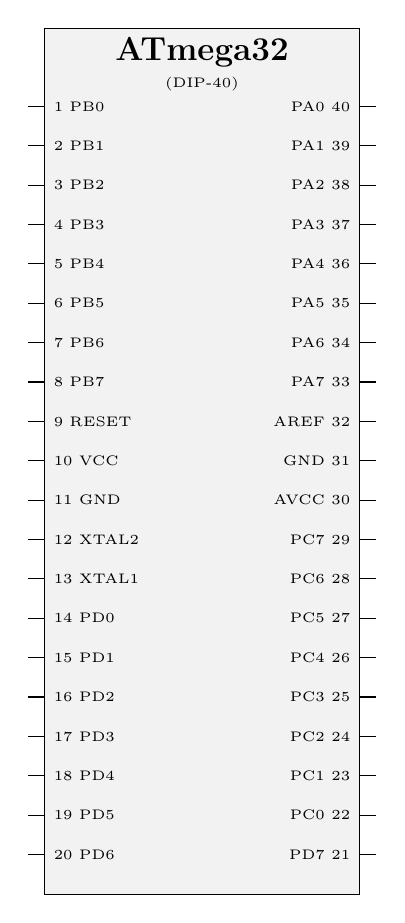
\begin{tikzpicture}[
    pin/.style={draw, rectangle, minimum width=2.5cm, minimum height=0.5cm, font=\small},
    ic/.style={draw, rectangle, minimum width=4cm, minimum height=11cm, fill=gray!10}
]
    % IC Body
    \node [ic] (body) {};
    \node [anchor=north, font=\large\bfseries] at (body.north) {ATmega32};
    \node [anchor=north] at (body.north) [yshift=-0.5cm] {\tiny (DIP-40)};

    % Left Pins
    \foreach \i/\label in {1/PB0, 2/PB1, 3/PB2, 4/PB3, 5/PB4, 6/PB5, 7/PB6, 8/PB7, 9/RESET, 10/VCC, 11/GND, 12/XTAL2, 13/XTAL1, 14/PD0, 15/PD1, 16/PD2, 17/PD3, 18/PD4, 19/PD5, 20/PD6} {
        \node [anchor=west, font=\tiny] at ([yshift=-0.5cm-\i*0.5cm]body.north west) {\i\ \label};
        \draw ([yshift=-0.5cm-\i*0.5cm]body.north west) -- +(-0.2,0);
    }

    % Right Pins
    \foreach \i/\label in {40/PA0, 39/PA1, 38/PA2, 37/PA3, 36/PA4, 35/PA5, 34/PA6, 33/PA7, 32/AREF, 31/GND, 30/AVCC, 29/PC7, 28/PC6, 27/PC5, 26/PC4, 25/PC3, 24/PC2, 23/PC1, 22/PC0, 21/PD7} {
        \pgfmathsetmacro{\ypos}{41-\i}
        \node [anchor=east, font=\tiny] at ([yshift=-0.5cm-\ypos*0.5cm]body.north east) {\label\ \i};
        \draw ([yshift=-0.5cm-\ypos*0.5cm]body.north east) -- +(0.2,0);
    }
\end{tikzpicture}
\end{center}
\end{solutionbox}

\begin{mnemonicbox}
\mnemonic{Port B A Reset Vcc Ground Crystal Port D C}
\end{mnemonicbox}

\questionmarks{2(b)}{4}{Explain status register of ATmega32.}

\begin{solutionbox}
\keyword{Status Register (SREG):}

\begin{answertable}{SREG Bit Configuration}
\begin{tabulary}{\linewidth}{|L|L|L|}
\hline
\textbf{Bit} & \textbf{Name} & \textbf{Function} \\ \hline
\keyword{Bit 7} & I & Global Interrupt Enable \\ \hline
\keyword{Bit 6} & T & Bit Copy Storage \\ \hline
\keyword{Bit 5} & H & Half Carry Flag \\ \hline
\keyword{Bit 4} & S & Sign Bit \\ \hline
\keyword{Bit 3} & V & Overflow Flag \\ \hline
\keyword{Bit 2} & N & Negative Flag \\ \hline
\keyword{Bit 1} & Z & Zero Flag \\ \hline
\keyword{Bit 0} & C & Carry Flag \\ \hline
\end{tabulary}
\end{answertable}

\keyword{Functions:}
\begin{itemize}
    \item \keyword{Flags Update}: Automatically set/cleared by ALU operations
    \item \keyword{Conditional Branching}: Used for program flow control (e.g., BREQ, BRCS)
    \item \keyword{Interrupt Control}: I-bit enables/disables all interrupts
\end{itemize}
\end{solutionbox}

\begin{mnemonicbox}
\mnemonic{I Think Half Sign Overflow Negative Zero Carry}
\end{mnemonicbox}

\questionmarks{2(c)}{7}{Explain data memory of ATmega32 in detail.}

\begin{solutionbox}
\textbf{Data Memory Organization:}

\begin{answerdiagram}{Data Memory Space}
\begin{tikzpicture}[auto, node distance=1.5cm]
    \node [gtu block, minimum width=4cm] (sram) {Data Memory Space};
    \node [gtu block, below=of sram] (gpr) {General Purpose Registers\\R0-R31 (0x00-0x1F)};
    \node [gtu block, below=of gpr] (io) {I/O Memory\\(0x20-0x5F)};
    \node [gtu block, below=of io] (extio) {Extended I/O\\(0x60-0xFF)};
    \node [gtu block, below=of extio] (ram) {Internal SRAM\\(0x100-0x8FF)};

    \path [gtu arrow] (sram) -- (gpr);
    \path [gtu arrow] (sram) edge[bend right] (io);
    \path [gtu arrow] (sram) edge[bend right] (extio);
    \path [gtu arrow] (sram) edge[bend right] (ram);
\end{tikzpicture}
\end{answerdiagram}

\keyword{Memory Sections:}
\begin{itemize}
    \item \keyword{General Purpose Registers}: 32 registers (R0-R31) for fast data operations, mapped to lowest addresses.
    \item \keyword{I/O Memory}: 64 registers for peripheral control (Port, Timer, UART, etc.), accessible via IN/OUT instructions.
    \item \keyword{Extended I/O}: Reserved for future use or extended peripheral control in some AVRs.
    \item \keyword{Internal SRAM}: 2KB (2048 bytes) of volatile memory for variables and stack.
    \item \keyword{Stack}: Implementation grows downward from high memory addresses towards low addresses.
\end{itemize}
\end{solutionbox}

\begin{mnemonicbox}
\mnemonic{General I/O Extended SRAM Address Stack}
\end{mnemonicbox}

\orquestionmarks{2(a)}{3}{Write functions of DDRx, PINx and PORTx registers.}

\begin{solutionbox}
\textbf{I/O Port Registers:}

\begin{answertable}{I/O Registers}
\begin{tabulary}{\linewidth}{|L|L|}
\hline
\textbf{Register} & \textbf{Function} \\ \hline
\keyword{DDRx} & Data Direction Register - configures pin direction \\ \hline
\keyword{PINx} & Pin Input Register - reads current pin logical state \\ \hline
\keyword{PORTx} & Port Output Register - writes data/pull-up control \\ \hline
\end{tabulary}
\end{answertable}

\keyword{Operations:}
\begin{itemize}
    \item \keyword{DDRx}: Set bit to 1 for Output, 0 for Input.
    \item \keyword{PINx}: Read accesses physical pin voltage level.
    \item \keyword{PORTx}: When DDRx=1, drives High/Low. When DDRx=0, enables internal Pull-up (if 1).
\end{itemize}
\end{solutionbox}

\begin{mnemonicbox}
\mnemonic{Direction Input Output}
\end{mnemonicbox}

\orquestionmarks{2(b)}{4}{Explain different I/O registers associated with EEPROM in AVR.}

\begin{solutionbox}
\keyword{EEPROM Registers:}

\begin{answertable}{EEPROM Registers}
\begin{tabulary}{\linewidth}{|L|L|}
\hline
\textbf{Register} & \textbf{Function} \\ \hline
\keyword{EEAR} & EEPROM Address Register (High/Low bytes) \\ \hline
\keyword{EEDR} & EEPROM Data Register \\ \hline
\keyword{EECR} & EEPROM Control Register \\ \hline
\end{tabulary}
\end{answertable}

\keyword{EECR Control Bits:}
\begin{itemize}
    \item \keyword{EERIE}: EEPROM Ready Interrupt Enable
    \item \keyword{EEMWE}: EEPROM Master Write Enable (Safety mechanism)
    \item \keyword{EEWE}: EEPROM Write Enable (Strobe to write)
    \item \keyword{EERE}: EEPROM Read Enable
\end{itemize}

\keyword{Process}: To write, ensure no write is in progress, set address and data, set EEMWE, then set EEWE within 4 clock cycles.
\end{solutionbox}

\begin{mnemonicbox}
\mnemonic{Address Data Control Ready Master Write Read}
\end{mnemonicbox}

\orquestionmarks{2(c)}{7}{Explain different ways of connecting clock sources to the AVR.}

\begin{solutionbox}
\textbf{Clock Source Options:}

\begin{answerdiagram}{Clock Sources}
\begin{tikzpicture}[auto, node distance=2cm]
    \node [gtu block] (avr) {AVR Microcontroller};
    \node [gtu block, above left=of avr] (xtal) {External Crystal\\(1-16 MHz)};
    \node [gtu block, below left=of avr] (extrc) {External RC\\Oscillator};
    \node [gtu block, above right=of avr] (intrc) {Internal RC\\(1, 2, 4, 8 MHz)};
    \node [gtu block, below right=of avr] (extclk) {External Clock\\Signal};

    \draw [gtu arrow] (xtal) -- (avr);
    \draw [gtu arrow] (extrc) -- (avr);
    \draw [gtu arrow] (intrc) -- (avr);
    \draw [gtu arrow] (extclk) -- (avr);
\end{tikzpicture}
\end{answerdiagram}

\begin{answertable}{Clock Source Types}
\begin{tabulary}{\linewidth}{|L|L|}
\hline
\textbf{Source} & \textbf{Description} \\ \hline
\keyword{External Crystal} & High precision quartz crystal connected to XTAL1/XTAL2. Capacitor needed. \\ \hline
\keyword{External RC} & Resistor-Capacitor circuit. Low cost, less precise. \\ \hline
\keyword{Internal RC} & Built-in oscillator. No external components. 1MHz default, up to 8MHz. \\ \hline
\keyword{External Clock} & Drive XTAL1 with external logic signal. \\ \hline
\end{tabulary}
\end{answertable}

\keyword{Configuration:}
\begin{itemize}
    \item \keyword{Fuse Bits}: CKSEL3:0 and SUT1:0 fuses determine the active clock source and startup time.
    \item \keyword{Usage}: Crystal for timing-critical (UART), Internal RC for cost/power saving.
\end{itemize}
\end{solutionbox}

\begin{mnemonicbox}
\mnemonic{Crystal RC Internal External Fuse Startup Frequency Components}
\end{mnemonicbox}

\questionmarks{3(a)}{3}{Write function of registers associated with Timer 1.}

\begin{solutionbox}
\textbf{Timer 1 Registers (16-bit):}

\begin{answertable}{Timer 1 Registers}
\begin{tabulary}{\linewidth}{|L|L|}
\hline
\textbf{Register} & \textbf{Function} \\ \hline
\keyword{TCNT1} & Timer/Counter Register - Holds current count value (16-bit) \\ \hline
\keyword{TCCR1A/B} & Control Registers - Sets mode, prescaler, compare output \\ \hline
\keyword{ICR1} & Input Capture Register - Captures TCNT1 value on event \\ \hline
\keyword{OCR1A/B} & Output Compare Registers - Values to compare with TCNT1 \\ \hline
\keyword{TIMSK} & Interrupt Mask - Enables Overflow/Compare/Capture interrupts \\ \hline
\keyword{TIFR} & Interrupt Flag - Indicates pending interrupts \\ \hline
\end{tabulary}
\end{answertable}
\end{solutionbox}

\begin{mnemonicbox}
\mnemonic{Timer Control Input Output Mask Flag}
\end{mnemonicbox}

\questionmarks{3(b)}{4}{Discuss steps to program Timer0 in Normal mode.}

\begin{solutionbox}
\textbf{Programming Steps used for Normal Mode:}

\begin{enumerate}
    \item \keyword{Configure Mode}: Write to TCCR0 to select Normal Mode (WGM01:0 = 00).
    \item \keyword{Load Initial Value}: Write starting count to TCNT0.
    \item \keyword{Interrupts}: If using interrupts, set TOIE0 in TIMSK and enable global interrupts (sei).
    \item \keyword{Start Timer}: Write non-zero prescaler value to Clock Select bits (CS02:0) in TCCR0.
    \item \keyword{Monitor/Handle}: Wait for TOV0 flag in TIFR (polling) or handle in ISR.
\end{enumerate}

\begin{lstlisting}[language=C]
TCCR0 = 0x00;        // Stop timer
TCNT0 = 0x00;        // Clear count
TCCR0 = 0x01;        // Start: Normal mode, No prescaler
while(!(TIFR & 1));  // Wait for overflow
TIFR = 0x01;         // Clear flag
\end{lstlisting}
\end{solutionbox}

\begin{mnemonicbox}
\mnemonic{Set Select Load Enable Start}
\end{mnemonicbox}

\questionmarks{3(c)}{7}{Write a C program to receive bytes of data serially and put them on PORT A. Set the baud rate at 9600, 8-bit, and 1 stop bit.}

\begin{solutionbox}
\textbf{Program:}

\begin{lstlisting}[language=C]
#include <avr/io.h>

void USART_Init() {
    // Set baud rate to 9600 (assuming 8MHz clock)
    // UBRR = (F_CPU / (16 * Baud)) - 1 = (8M / (16 * 9600)) - 1 = 51
    UBRRH = 0x00;
    UBRRL = 51;
    
    // Enable receiver
    UCSRB = (1<<RXEN);
    
    // Set frame format: 8 data, 1 stop bit
    // URSEL must be 1 to write to UCSRC
    UCSRC = (1<<URSEL) | (3<<UCSZ0);
}

unsigned char USART_Receive() {
    // Wait for data to be received (RXC flag)
    while(!(UCSRA & (1<<RXC)));
    // Get and return received data from buffer
    return UDR;
}

int main() {
    DDRA = 0xFF;        // Configure PORTA as output
    USART_Init();       // Initialize USART
    
    while(1) {
        PORTA = USART_Receive();  // Receive and display on Port A
    }
    return 0;
}
\end{lstlisting}

\keyword{Configuration Details:}
\begin{itemize}
    \item \keyword{Baud Rate}: 9600 bps requires UBRR=51 at 8MHz.
    \item \keyword{Frame Format}: 8-bit data (UCSZ1:0 = 11), 1 stop bit (USBS = 0).
    \item \keyword{Reception}: Polling RXC bit in UCSRA ensures valid data is read.
\end{itemize}
\end{solutionbox}

\begin{mnemonicbox}
\mnemonic{Initialize Receive Display Loop}
\end{mnemonicbox}

\orquestionmarks{3(a)}{3}{Write function of registers associated with Serial Communication in AVR.}

\begin{solutionbox}
\textbf{USART Registers:}

\begin{answertable}{USART Registers}
\begin{tabulary}{\linewidth}{|L|L|}
\hline
\textbf{Register} & \textbf{Function} \\ \hline
\keyword{UDR} & USART Data Register - Buffer for Tx/Rx data \\ \hline
\keyword{UCSRA} & Control/Status A - Flags (RXC, TXC, UDRE), error bits \\ \hline
\keyword{UCSRB} & Control/Status B - Enable Rx/Tx, Interrupts (RXCIE), 9th bit \\ \hline
\keyword{UCSRC} & Control/Status C - Frame format (Data bits, Parity, Stop bits) \\ \hline
\keyword{UBRR} & Baud Rate Register - Sets communication speed \\ \hline
\end{tabulary}
\end{answertable}
\end{solutionbox}

\begin{mnemonicbox}
\mnemonic{Data Control Status Baud}
\end{mnemonicbox}

\orquestionmarks{3(b)}{4}{Discuss steps to program AVR to transfer data serially.}

\begin{solutionbox}
\textbf{Steps for Serial Transmission:}

\begin{enumerate}
    \item \keyword{Baud Rate}: Calculate and load value into UBRRH/Low registers.
    \item \keyword{Frame Format}: Set data bits, parity, and stop bits in UCSRC (e.g., 8N1).
    \item \keyword{Enable Tx}: Set TXEN bit in UCSRB to enable transmitter.
    \item \keyword{Wait for Buffer}: Monitor UDRE flag in UCSRA to ensure UDR is empty.
    \item \keyword{Send Data}: Write byte to UDR register to start transmission.
\end{enumerate}

\begin{lstlisting}[language=C]
void USART_Transmit(unsigned char data) {
    // Wait for empty transmit buffer
    while(!(UCSRA & (1<<UDRE)));
    // Put data into buffer, sends the data
    UDR = data;
}
\end{lstlisting}
\end{solutionbox}

\begin{mnemonicbox}
\mnemonic{Baud Enable Format Wait Load}
\end{mnemonicbox}

\orquestionmarks{3(c)}{7}{Write a C program to toggle only the PORTB.4 bit continuously every 2 ms. Use timer 1, Normal mode, and no prescaler to create the delay. Assume XTAL=8MHz.}

\begin{solutionbox}
\textbf{Timer 1 Delay Calculation:}
\begin{itemize}
    \item \keyword{Target Delay}: 2 ms
    \item \keyword{Frequency}: 8 MHz
    \item \keyword{Machine Cycle}: $1/8\text{MHz} = 0.125\mu\text{s}$
    \item \keyword{Counts Required}: $2\text{ms} / 0.125\mu\text{s} = 16000$ counts
    \item \keyword{Timer Start Value}: $65536 - 16000 = 49536$ (0xC180)
\end{itemize}

\textbf{Program:}

\begin{lstlisting}[language=C]
#include <avr/io.h>
#include <avr/interrupt.h>

// ISR for Timer1 Overflow
ISR(TIMER1_OVF_vect) {
    // Toggle PORTB.4
    PORTB ^= (1<<4);
    
    // Reload Timer for 2ms
    TCNT1 = 49536; 
}

int main() {
    // Set PORTB.4 as output
    DDRB |= (1<<4);
    
    // Initialize Timer1
    // Normal Mode (WGM13:0 = 0000)
    TCCR1A = 0x00;
    
    // Start Timer with No Prescaler (CS12:0 = 001)
    TCCR1B = (1<<CS10);
    
    // Load initial count
    TCNT1 = 49536;
    
    // Enable Timer1 Overflow Interrupt
    TIMSK |= (1<<TOIE1);
    
    // Enable Global Interrupts
    sei();
    
    while(1) {
        // Main loop does nothing, ISR handles toggling
    }
    return 0;
}
\end{lstlisting}
\end{solutionbox}

\begin{mnemonicbox}
\mnemonic{Configure Timer Calculate Enable Loop}
\end{mnemonicbox}

\questionmarks{4(a)}{3}{Draw interfacing diagram of ULN2803 with ATmega32.}

\begin{solutionbox}
\textbf{ULN2803 Interfacing:}

\begin{answerdiagram}{ULN2803 Interface}
\begin{tikzpicture}[auto, node distance=1.5cm]
    \node [gtu block, minimum height=2.5cm] (mcu) {ATmega32\\PORTB};
    \node [gtu block, right=of mcu, minimum height=2.5cm] (uln) {ULN2803\\Driver};
    \node [gtu block, right=of uln, minimum height=2cm] (load) {Loads\\(Relay/Motor)};
    
    \draw [gtu arrow] (mcu.20) -- node[above, font=\tiny] {PB0} (uln.160);
    \draw [gtu arrow] (mcu.0) -- node[above, font=\tiny] {PB1} (uln.180);
    \draw [gtu arrow] (mcu.-20) -- node[above, font=\tiny] {PB2} (uln.200);
    
    \draw [gtu arrow] (uln.20) -- node[above, font=\tiny] {OUT1} (load.160);
    \draw [gtu arrow] (uln.0) -- node[above, font=\tiny] {OUT2} (load.180);
    \draw [gtu arrow] (uln.-20) -- node[above, font=\tiny] {OUT3} (load.200);
    
    \node [above=0.5cm of load] (vcc) {+12V};
    \draw [gtu arrow] (vcc) -- (load);
    \draw [gtu arrow] (uln.270) -- ++(0,-0.5) node[below] {GND};
    \draw [gtu arrow] (uln.90) -- ++(0,0.5) node[above] {COM (+12V)};
\end{tikzpicture}
\end{answerdiagram}

\keyword{Connections:}
\begin{itemize}
    \item \keyword{Inputs}: Connect ATmega32 pins directly to ULN2803 inputs (1B-8B).
    \item \keyword{Outputs}: Open collector outputs drive loads connected to positive supply.
    \item \keyword{Common}: Pin 10 to COM (Load Supply) for flyback diodes, Pin 9 to GND.
\end{itemize}
\end{solutionbox}

\begin{mnemonicbox}
\mnemonic{Input Output Common Supply Ground}
\end{mnemonicbox}

\questionmarks{4(b)}{4}{Write an AVR C program to get a byte of data from Port B, and then send it to Port C.}

\begin{solutionbox}
\textbf{Program:}

\begin{lstlisting}[language=C]
#include <avr/io.h>

int main() {
    // Configure Directions
    DDRB = 0x00;    // Port B as Input
    DDRC = 0xFF;    // Port C as Output
    
    // Enable Pull-ups on Input Port
    PORTB = 0xFF;   
    
    while(1) {
        // Read data from PINB register
        unsigned char data = PINB;
        
        // Write data to PORTC register
        PORTC = data;
    }
    return 0;
}
\end{lstlisting}

\begin{itemize}
    \item \keyword{Direction}: DDRB=0 (In), DDRC=1 (Out).
    \item \keyword{Pull-ups}: Writing 1 to PORTB when DDRB=0 enables internal pull-ups.
    \item \keyword{Transfer}: Continuous loop reads PINB and updates PORTC.
\end{itemize}
\end{solutionbox}

\begin{mnemonicbox}
\mnemonic{Configure Enable Read Write}
\end{mnemonicbox}

\questionmarks{4(c)}{7}{Draw and explain interfacing of MAX7221 with ATmega32.}

\begin{solutionbox}
\textbf{MAX7221 Interface:}

\begin{answerdiagram}{MAX7221 Interface}
\begin{tikzpicture}[auto, node distance=2cm]
    \node [gtu block] (mcu) {ATmega32};
    \node [gtu block, right=of mcu] (max) {MAX7221\\Display Driver};
    \node [gtu block, right=of max, align=center] (disp) {7-Segment\\Display};
    
    \draw [gtu arrow] (mcu.20) -- node[above, font=\tiny] {PB5 (MOSI)} (max.160);
    \draw [gtu arrow] (mcu.0) -- node[above, font=\tiny] {PB7 (SCK)} (max.180);
    \draw [gtu arrow] (mcu.-20) -- node[above, font=\tiny] {PB4 (SS)} (max.200);
    
    \draw [gtu arrow] (max) -- node[above, font=\tiny] {SEG/DIG} (disp);
    
    \node [above=0.3cm of max] (vcc) {VCC};
    \draw [gtu arrow] (vcc) -- (max);
\end{tikzpicture}
\end{answerdiagram}

\keyword{Interface Details:}
\begin{itemize}
    \item \keyword{Protocol}: SPI (Serial Peripheral Interface). 3-wire: Data (DIN), Clock (CLK), Load (CS).
    \item \keyword{Function}: Drives up to 8 common-cathode 7-segment displays.
    \item \keyword{Multiplexing}: Handles scanning circuitry internally.
    \item \keyword{Current Control}: Set via external resistor (ISET pin).
\end{itemize}

\keyword{Programming}:
\begin{enumerate}
    \item Pull LOAD (CS) Low.
    \item Shift in 16-bit word (Address + Data) via DIN on CLK rising edge.
    \item Pulse LOAD High to latch data.
\end{enumerate}
\end{solutionbox}

\begin{mnemonicbox}
\mnemonic{SPI Data Clock Load Multiplex Current Program}
\end{mnemonicbox}

\orquestionmarks{4(a)}{3}{Draw interfacing diagram of LM35 with ATmega32.}

\begin{solutionbox}
\textbf{LM35 Interface Circuit:}

\begin{answerdiagram}{LM35 Connection}
\begin{tikzpicture}[auto, node distance=2cm]
    \node [gtu block] (lm35) {LM35\\Sensor};
    \node [gtu block, right=of lm35] (mcu) {ATmega32\\(ADC)};
    
    \draw [gtu arrow] (lm35) -- node[midway, above] {Vout} node[midway, below] {(10mV/$^\circ$C)} (mcu);
    
    \node [above=0.5cm of lm35] (vcc) {+5V};
    \node [below=0.5cm of lm35] (gnd) {GND};
    \draw [gtu arrow] (vcc) -- (lm35);
    \draw [gtu arrow] (lm35) -- (gnd);
    
    \node [right=0.1cm of mcu] (adc) {PA0 (ADC0)};
\end{tikzpicture}
\end{answerdiagram}

\keyword{Specifications:}
\begin{itemize}
    \item \keyword{Output}: Linear voltage proportional to temperature ($10\text{mV}/^\circ\text{C}$).
    \item \keyword{Connection}: Vout connected to any ADC channel (e.g., PA0).
    \item \keyword{Conversion}: $V_{in} \times \frac{1024}{V_{ref}} = \text{ADC Value}$.
\end{itemize}
\end{solutionbox}

\begin{mnemonicbox}
\mnemonic{VCC OUT GND Linear}
\end{mnemonicbox}

\orquestionmarks{4(b)}{4}{Write an AVR C program to monitor bit 5 of port C, if it is HIGH, send 55H to Port B; otherwise, send AAH to Port B.}

\begin{solutionbox}
\textbf{Program:}

\begin{lstlisting}[language=C]
#include <avr/io.h>

int main() {
    DDRC &= ~(1<<5);    // PC5 as Input
    PORTC |= (1<<5);    // Enable Pull-up on PC5
    DDRB = 0xFF;        // Port B as Output
    
    while(1) {
        // Check if PC5 is High
        if(PINC & (1<<5)) {
            PORTB = 0x55;   // Pattern 01010101
        } else {
            PORTB = 0xAA;   // Pattern 10101010
        }
    }
    return 0;
}
\end{lstlisting}

\keyword{Logic:}
\begin{itemize}
    \item \keyword{Masking}: \code{PINC \& (1<<5)} isolates bit 5.
    \item \keyword{Condition}: If result is non-zero (True), bit is High.
\end{itemize}
\end{solutionbox}

\begin{mnemonicbox}
\mnemonic{Monitor Conditional Output Loop}
\end{mnemonicbox}

\orquestionmarks{4(c)}{7}{Discuss registers used to program SPI in the AVR.}

\begin{solutionbox}
\keyword{SPI Registers:}

\begin{answertable}{SPI Registers}
\begin{tabulary}{\linewidth}{|L|L|}
\hline
\textbf{Register} & \textbf{Function} \\ \hline
\keyword{SPCR} & Control Register - EN, Int, Order, Master/Slave, Mode \\ \hline
\keyword{SPSR} & Status Register - Interrupt Flag (SPIF), Collision (WCOL) \\ \hline
\keyword{SPDR} & Data Register - Shift register for transmission/reception \\ \hline
\end{tabulary}
\end{answertable}

\keyword{SPCR Bits:}
\begin{itemize}
    \item \keyword{SPE}: SPI Enable.
    \item \keyword{MSTR}: Master (1) or Slave (0) Select.
    \item \keyword{SPR1:0}: Clock Rate Select (fosc/4, /16, /64, /128).
    \item \keyword{CPOL/CPHA}: Clock Polarity and Phase (Mode 0-3).
\end{itemize}

\keyword{Usage}: Write to SPDR starts transmission (Master). Read SPDR after SPIF is set retrieves received data.
\end{solutionbox}

\begin{mnemonicbox}
\mnemonic{Control Status Data Configure Enable Write Wait Read}
\end{mnemonicbox}

\questionmarks{5(a)}{3}{Draw pin diagram of L293D motor driver IC.}

\begin{solutionbox}
\textbf{L293D Pinout:}

\begin{center}
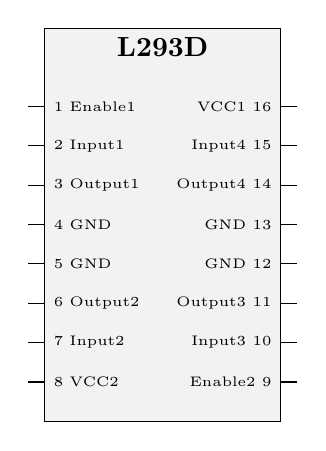
\begin{tikzpicture}[
    pin/.style={draw, rectangle, minimum width=2cm, minimum height=0.5cm, font=\tiny},
    ic/.style={draw, rectangle, minimum width=3cm, minimum height=5cm, fill=gray!10}
]
    \node [ic] (body) {};
    \node [anchor=north, font=\bfseries] at (body.north) {L293D};

    % Pins Left
    \foreach \i/\label in {1/Enable1, 2/Input1, 3/Output1, 4/GND, 5/GND, 6/Output2, 7/Input2, 8/VCC2} {
        \node [anchor=west, font=\tiny] at ([yshift=-0.5cm-\i*0.5cm]body.north west) {\i\ \label};
        \draw ([yshift=-0.5cm-\i*0.5cm]body.north west) -- +(-0.2,0);
    }

    % Pins Right
    \foreach \i/\label in {16/VCC1, 15/Input4, 14/Output4, 13/GND, 12/GND, 11/Output3, 10/Input3, 9/Enable2} {
        \pgfmathsetmacro{\ypos}{17-\i}
        \node [anchor=east, font=\tiny] at ([yshift=-0.5cm-\ypos*0.5cm]body.north east) {\label\ \i};
        \draw ([yshift=-0.5cm-\ypos*0.5cm]body.north east) -- +(0.2,0);
    }
\end{tikzpicture}
\end{center}
\end{solutionbox}

\begin{mnemonicbox}
\mnemonic{Enable Input Output Supply Ground}
\end{mnemonicbox}

\questionmarks{5(b)}{4}{Draw and explain ADMUX register.}

\begin{solutionbox}
\keyword{ADMUX (ADC Multiplexer Selection Register):}

\begin{answertable}{ADMUX Register}
\begin{tabulary}{\linewidth}{|c|c|c|c|c|c|c|c|}
\hline
\textbf{7} & \textbf{6} & \textbf{5} & \textbf{4} & \textbf{3} & \textbf{2} & \textbf{1} & \textbf{0} \\ \hline
REFS1 & REFS0 & ADLAR & MUX4 & MUX3 & MUX2 & MUX1 & MUX0 \\ \hline
\end{tabulary}
\end{answertable}

\keyword{Bit Descriptions:}
\begin{itemize}
    \item \keyword{REFS1:0}: Reference Selection Bits.
        \begin{itemize}
            \item 00: AREF, Internal Vref turned off.
            \item 01: AVCC with external capacitor at AREF pin.
            \item 11: Internal 2.56V Voltage Reference.
        \end{itemize}
    \item \keyword{ADLAR}: ADC Left Adjust Result. If 1, result is left-adjusted (for 8-bit precision).
    \item \keyword{MUX4:0}: Analog Channel and Gain Selection Bits. Selects which ADC pin (ADC0-ADC7) is connected to the ADC.
\end{itemize}
\end{solutionbox}

\begin{mnemonicbox}
\mnemonic{Reference Adjust Multiplex Channel}
\end{mnemonicbox}

\questionmarks{5(c)}{7}{Explain the block diagram of GSM based security system.}

\begin{solutionbox}
\textbf{GSM Security System:}

\begin{answerdiagram}{GSM Security Block Diagram}
\begin{tikzpicture}[auto, node distance=2cm]
    \node [gtu block] (mcu) {Microcontroller\\(ATmega32)};
    \node [gtu input, left=of mcu] (sensor) {Sensors\\(PIR/Door)};
    \node [gtu block, right=of mcu] (gsm) {GSM Module\\(SIM900)};
    \node [gtu block, above=of mcu] (lcd) {LCD Display};
    \node [gtu block, below=of mcu] (alarm) {Alarm/Buzzer};
    \node [gtu block, right=of gsm] (network) {Mobile\\Network};
    \node [gtu block, below=of network] (user) {User Phone};

    \draw [gtu arrow] (sensor) -- (mcu);
    \draw [gtu arrow] (mcu) -- (gsm);
    \draw [gtu arrow] (mcu) -- (lcd);
    \draw [gtu arrow] (mcu) -- (alarm);
    \draw [gtu arrow] (gsm) -- (network);
    \draw [gtu arrow] (network) -- (user);
\end{tikzpicture}
\end{answerdiagram}

\keyword{System Components:}
\begin{itemize}
    \item \keyword{Sensors}: PIR sensor detects motion, Door switches detect entry.
    \item \keyword{Microcontroller}: Processes sensor inputs. If intrusion detected:
        \begin{enumerate}
            \item Activates Alarm/Buzzer.
            \item Sends AT commands to GSM Module.
            \item Updates Status on LCD.
        \end{enumerate}
    \item \keyword{GSM Module}: Communicates with cellular network via UART. Sends SMS/Call to user.
    \item \keyword{User Mobile}: Receives alert ("Intruder Detected!").
\end{itemize}
\end{solutionbox}

\begin{mnemonicbox}
\mnemonic{Sensors Microcontroller GSM Mobile Alarm Display Power Operation}
\end{mnemonicbox}

\orquestionmarks{5(a)}{3}{Draw circuit diagram to interface DC motor with ATmega32 using L293D motor driver.}

\begin{solutionbox}
\textbf{DC Motor Interface:}

\begin{answerdiagram}{DC Motor with L293D}
\begin{tikzpicture}[auto, node distance=2cm]
    \node [gtu block] (mcu) {ATmega32};
    \node [gtu block, right=of mcu] (l293) {L293D};
    \node [gtu block, right=of l293] (motor) {DC Motor};
    
    \draw [gtu arrow] (mcu.30) -- node[above, font=\tiny] {PB0(EN)} (l293.150);
    \draw [gtu arrow] (mcu.0) -- node[above, font=\tiny] {PB1(IN1)} (l293.180);
    \draw [gtu arrow] (mcu.-30) -- node[above, font=\tiny] {PB2(IN2)} (l293.210);
    
    \draw [gtu arrow] (l293.30) -- node[above, font=\tiny] {OUT1} (motor.150);
    \draw [gtu arrow] (l293.-30) -- node[above, font=\tiny] {OUT2} (motor.210);
    
    \node [above=0.5cm of l293] (vcc) {VCC (5V/12V)};
    \draw [gtu arrow] (vcc) -- (l293);
\end{tikzpicture}
\end{answerdiagram}

\keyword{Control Logic:}
\begin{itemize}
    \item \keyword{Enable}: High (1) to activate driver channel.
    \item \keyword{Direction}: IN1=1, IN2=0 (Forward); IN1=0, IN2=1 (Reverse).
    \item \keyword{Stop}: IN1=0, IN2=0.
\end{itemize}
\end{solutionbox}

\begin{mnemonicbox}
\mnemonic{Enable Direction Output Power Control}
\end{mnemonicbox}

\orquestionmarks{5(b)}{4}{Draw and explain ADCSRA register.}

\begin{solutionbox}
\keyword{ADCSRA (ADC Control and Status Register A):}

\begin{answertable}{ADCSRA Register}
\begin{tabulary}{\linewidth}{|c|c|c|c|c|c|c|c|}
\hline
\textbf{7} & \textbf{6} & \textbf{5} & \textbf{4} & \textbf{3} & \textbf{2} & \textbf{1} & \textbf{0} \\ \hline
ADEN & ADSC & ADATE & ADIF & ADIE & ADPS2 & ADPS1 & ADPS0 \\ \hline
\end{tabulary}
\end{answertable}

\keyword{Bit Functions:}
\begin{itemize}
    \item \keyword{ADEN}: ADC Enable. Must be set to 1 to use ADC.
    \item \keyword{ADSC}: Start Conversion. Write 1 to start a single conversion.
    \item \keyword{ADATE}: Auto Trigger Enable.
    \item \keyword{ADIF}: Interrupt Flag. Set when conversion completes.
    \item \keyword{ADIE}: Interrupt Enable. Activates ADC interrupt if Global Interrupts are enabled.
    \item \keyword{ADPS2:0}: Prescaler Select. Divides system clock (e.g., /128 for 8MHz crystal) to get ADC clock (50-200kHz).
\end{itemize}
\end{solutionbox}

\begin{mnemonicbox}
\mnemonic{Enable Start Auto Interrupt Prescaler Configure}
\end{mnemonicbox}

\end{document}
